\section{Systematics}
\label{sec:systematics}

The expected number of signal events in this analysis is projected with Monte Carlo simulation.
Possible differences between data reconstruction and Monte Carlo reconstruction are usually corrected with data/Monte Carlo scale factors.
In this analysis, the systematics related to those differences come in two possible categories: normalization uncertanties and shape uncertainties.
The normalization systematics are related to the uncertainty in the expected number of signal events. This is due to different efficiencies of the analysis selections in data and Monte Carlo reconstructions.
Shape systematics are important in this analysis because the signal shapes enter the signal extraction procedure in the parametric fits. Therefore, uncertainties in the shape of $\Mgg$ and $\Mjj$ distributions must be included as systematics.

Both normalization and shape uncertainties come from photons and jets.
Since the photons in this analysis are selected with the same selection criteria as the SM $\Hgg$ analysis, we take the photon related systematics from that.
This includes the photon energy scale (PES) and photon energy resolution (PER).
These two uncertainties are translated into two shape systematics ($\Delta\Mgg/\Mgg$ and $\Delta \sigma_{\Mgg}/\sigma_{\Mgg}$), and into the photon selection selection acceptance uncertainty (which inclues the trigger pre-selection requirements).
The PES has to cover as well effects of linearity in the energy scale for high $E_{T}$. For this, $\Delta\Mgg/\Mgg$ is kept at $0.7\%$ (cite diphoton high mass moriond PAS) for 2015 and  $0.05\%$ for 2016 (cite Hgg presentation on Higgs recap).

For jets, the jet energy scale (JES) and jet energy resolution (JER) are important ingredients in the list of systematics.
As for photons, they enter in the analysis in two shape systematics ($\Delta\Mjj/\Mjj$ and $\Delta \sigma_{\Mjj}/\sigma_{\Mjj}$), and in the jet selection acceptance uncertainty (related to the jet kinematic requirements).
An extra jet related systematic is related to the b-tagging requirements. The analysis has defined four b-tagging regions in total (two for resonant and two for non-resonant); for each one, the uncertainty of the b-tagging efficiency must be taken into account.

An extra set of normalization systematics are needed because of the mass window requirement in the resonant analysis.
This systematic is related to the change in signal efficiency after variations of PES/PER/JES/JER.

A systematic due to the uncertainty in the integrated luminosity measurement in CMS is included.

No theory systematics are applied to our BSM signals.

The values of those quantities are shown in table \ref{tab:sys} for 2015 data and will be updated with 2016 values.

\begin{table}[h]
\renewcommand{\arraystretch}{1.1}
\centering
{\small
\begin{tabular}{|l r|c|}
\hline
{\bf Sources of Systematical Uncertainties} & Type & Value  \\ \hline \hline
\multicolumn{3}{|c|}{General uncertainties} \\
\hline
Integrated luminosity & Normalization & 2.7\%  \\
%Diphoton trigger efficiency & 1.0\% \\
\hline
\hline
\multicolumn{3}{|c|}{Photon related uncertainties} \\\hline
Photon energy scale ($\frac{\Delta \Mgg}{\Mgg}$) & Shape & $1.0\%$  \\
Photon energy resolution ($\frac{\Delta \sigma_{\gamma\gamma}}{\sigma_{\gamma\gamma}}$) & Shape & $1.0\%$  \\
Diphoton pre-selection (with trigger uncertainties) & Normalization &$2.0\%$   \\ 
Photon Identification & Normalization & $1.0\%$  \\
%Acceptance in $\pTj$ ( JES and JER) & $1.0\%$\\

\hline \multicolumn{3}{|c|}{Jet related uncertainties} \\\hline
Jet energy scale ($\frac{\Delta \Mjj}{\Mjj}$) & Shape & $2.0\%$  \\
Jet energy resolution ($\frac{\Delta \sigma_{jj}}{\sigma_{jj}}$) & Shape & $8.0\%$  \\

\hline \multicolumn{3}{|c|}{Resonant specific uncertainties} \\\hline
Mass window selection (with jet selection uncertainty) & Normalization & $5.0\%$  \\
\PQb tagging efficiency (Low Mass, high purity) & Normalization & $2.5\%$  \\ 
\PQb tagging efficiency (Low Mass, medium purity) & Normalization & $1.0\%$  \\ 
\PQb tagging efficiency (High Mass) & Normalization & $1.0\%$  \\

\hline \multicolumn{3}{|c|}{Nonresonant specific uncertainties} \\\hline
Jet Selection plus $\Mtilde > 350 $ GeV & Normalization & $3.0\%$  \\ 
%Jet Selection plus $\Mtilde < 350 $ GeV (low mass category) & Normalization & $3\%$  \\ \hline
\PQb tagging efficiency (high purity) & Normalization & $4.5\%$   \\ 
\PQb tagging efficiency (medium purity) & Normalization & $1.0\%$   \\ \hline
\end{tabular}
}
%{\bf FIXME: table from Run I paper} 
%\url{https://twiki.cern.ch/twiki/bin/view/LHCPhysics/LHCHXSWGHH#Current_recommendations_for_di_H}
\caption{\small 
Summary of systematic uncertainties. The uncertainty in the \PQb tagging efficiency is anticorrelated between the \PQb tag categories.}
\label{tab:sys}
\end{table}  


\subsection{Signal shape smearings}

One important ingredient when applying the analysis systematics is the smearing of the signal shapes. 
After the signal model is fitted to the signal simulation, all PDF parameters are fixed. 
Following, the signal mean and width are then multiplied by smearing factors related to scale and resolution uncertainties, respectively. 
While this is clearly un-problematic for the mean, since it merely causes a scaling of the x axis, this might not be the case for the resolution smearing. 
In the latter case, the tail parameters of the signal modeling can be affected by the smearing and not correspond to the frozen parameters from the pre-smearing fit. 
To test this, we fit the smeared MC (MC with photon and jet energy resolution smearing uncertainty values applied) with the signal PDF with the tails fixed to their values from the un-smeared MC (MC with central values of smearings) and we compare with the smeared MC fit with the signal PDF without fixing the tail parameters - these different fits are shown in Figures \ref{fig:mgg_smear} and \ref{fig:mjj_smear}.
We have also compared the 2D residuals (as defined in the Signal Model section) of the fixed tails PDF vs the smeared MC with the floating tails PDF vs the smeared MC, shown in Figure \ref{fig:res_smear}.  
Additionally, we compare the fixed and floating fit shapes in Figure \ref{fig:comp_smear}.
Since no issue has been seen, we continue using the procedure described in the previous section for applying the signal smearing.

 
\begin{figure*}[h]
  \centering
  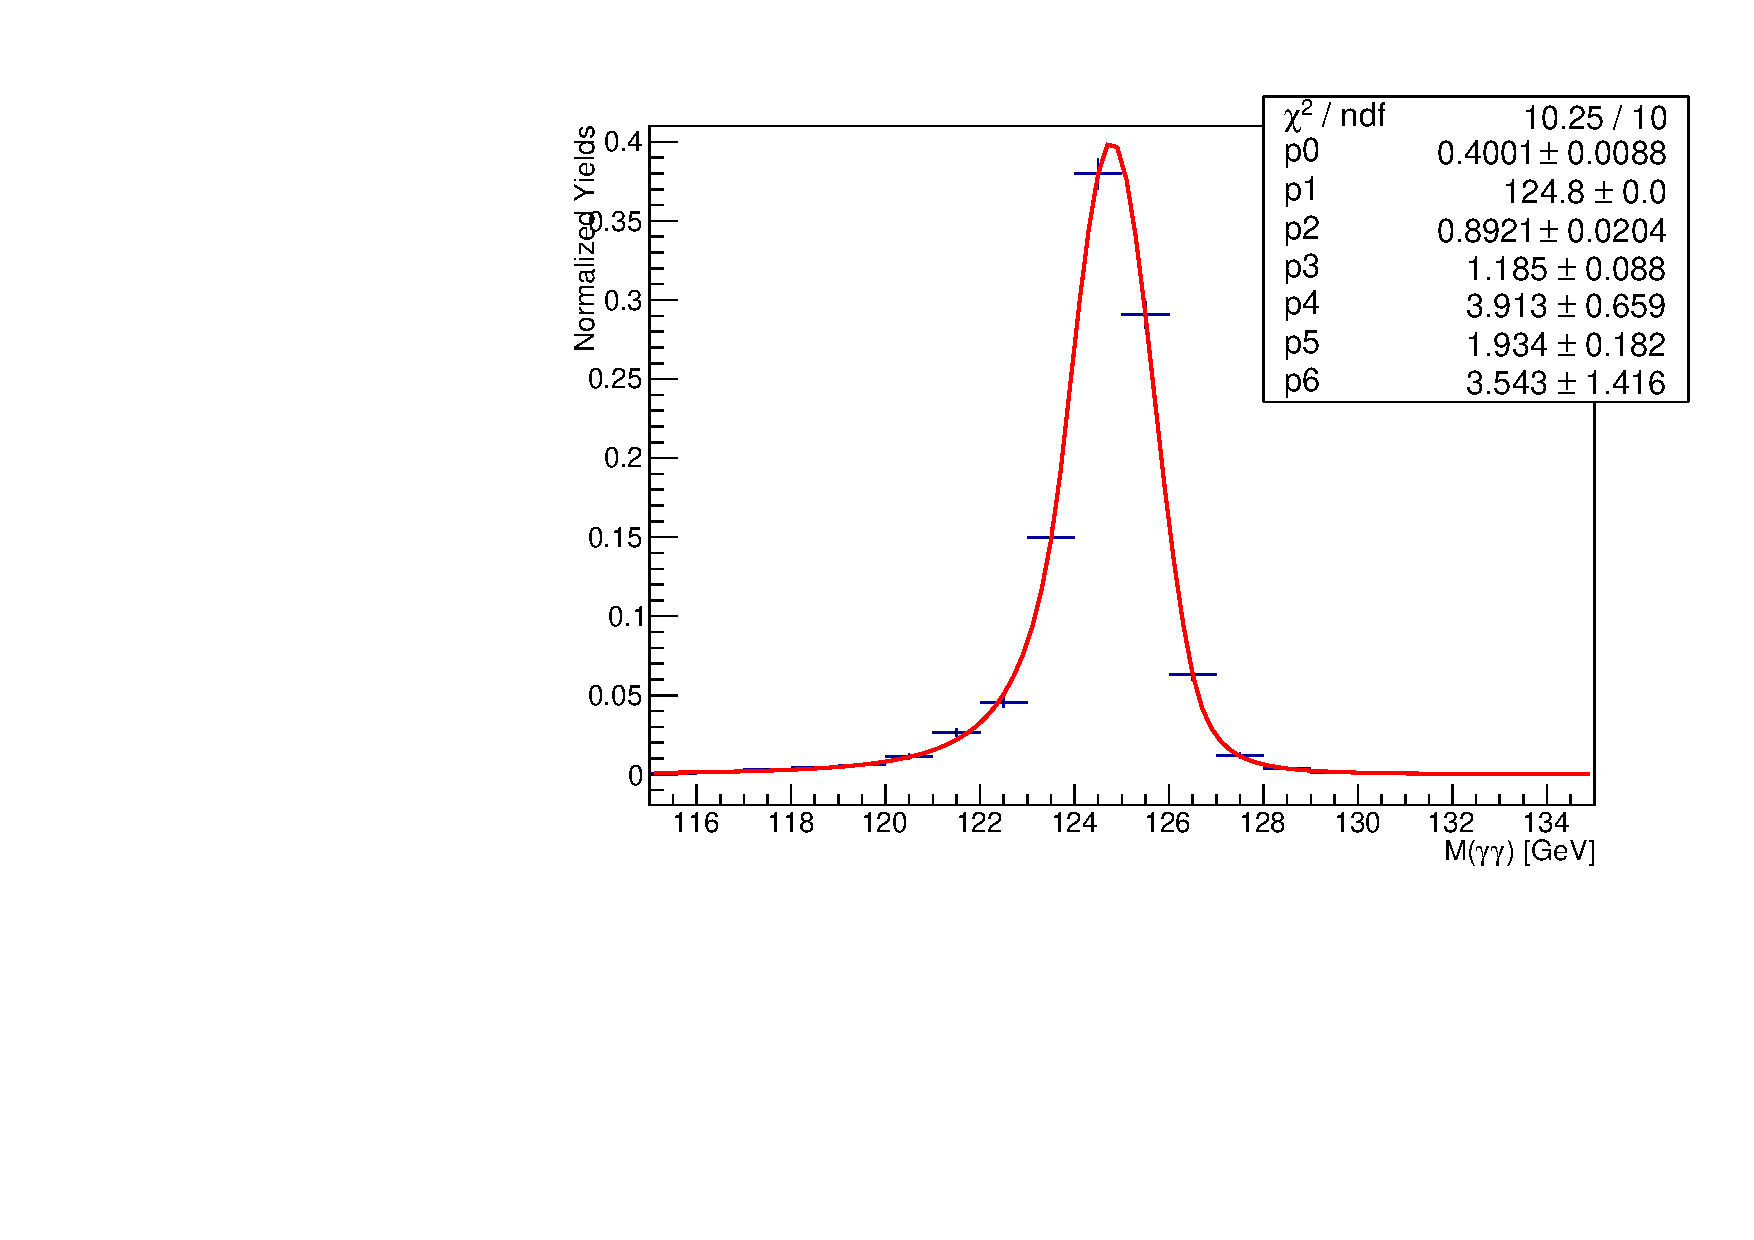
\includegraphics[width=0.45\textwidth]{figures/sec-systematics/mggHMMPC_floating_central.pdf}\hfil
  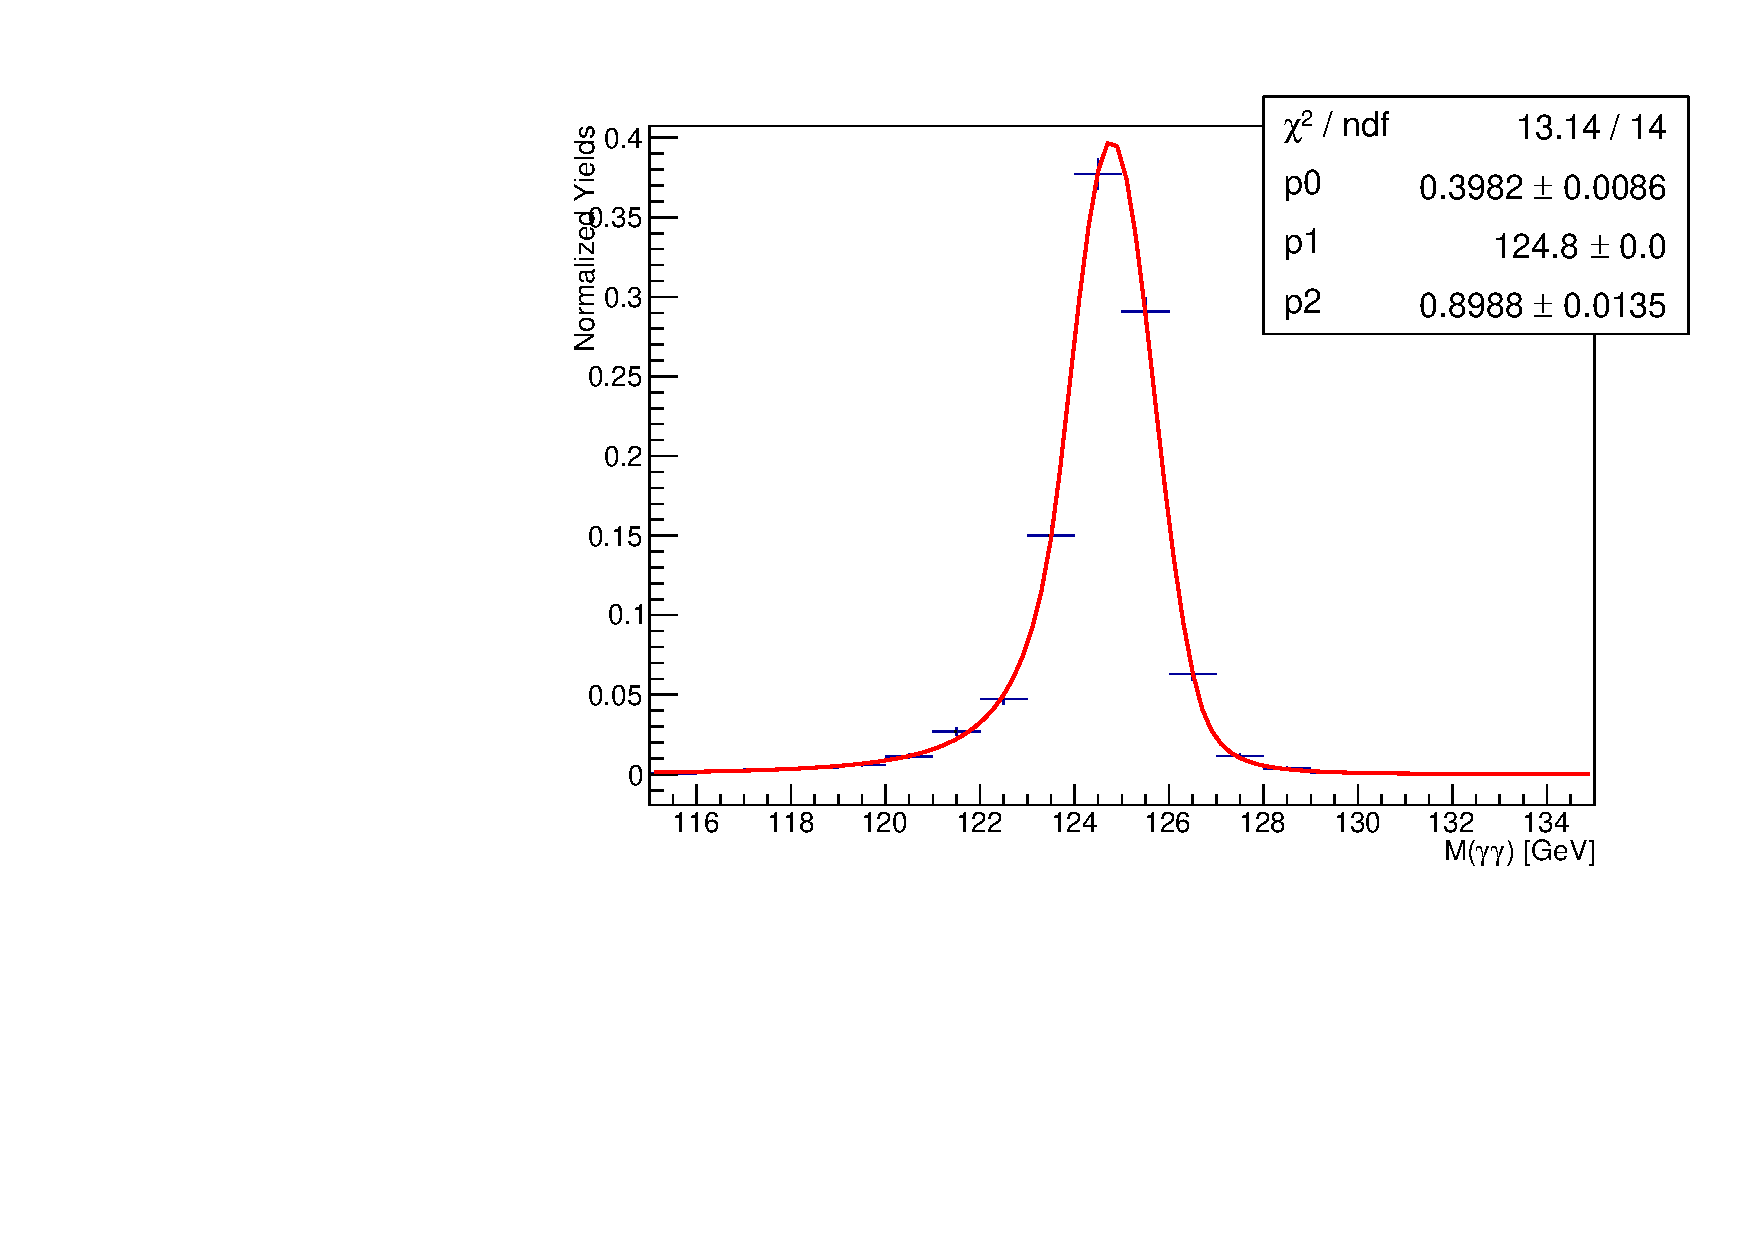
\includegraphics[width=0.45\textwidth]{figures/sec-systematics/mggHMMPC_fixed_up.pdf}\hfil
  \caption{Signal fits for the High Mass Medium purity categories, in the un-smeared MC with floating tails (left) and on the smeared MC with fixed tails (right). The tail parameters on the right are fixed to their values on the left.}
  \label{fig:mgg_smear}
\end{figure*}

\begin{figure*}[h]
  \centering
  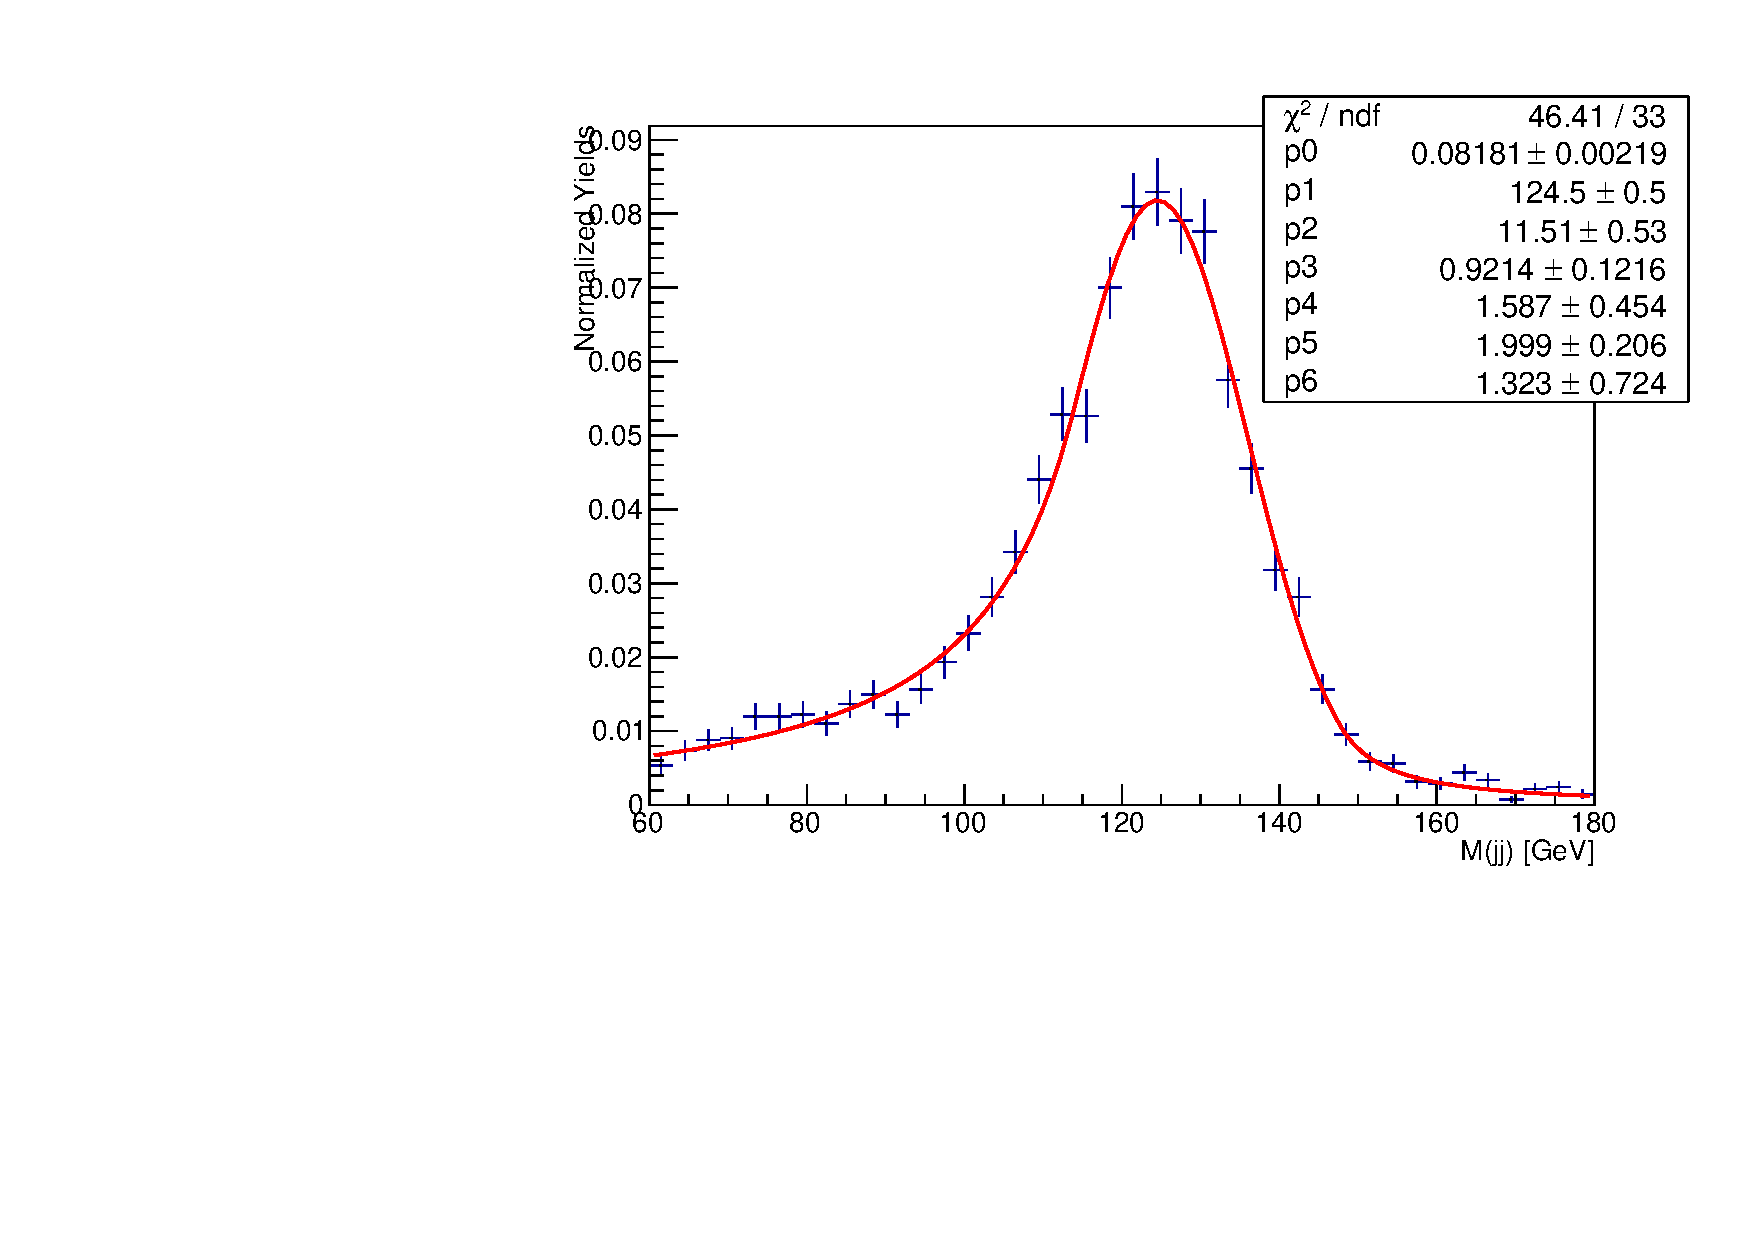
\includegraphics[width=0.45\textwidth]{figures/sec-systematics/mjjHMMPC_floating_central.pdf}\hfil
  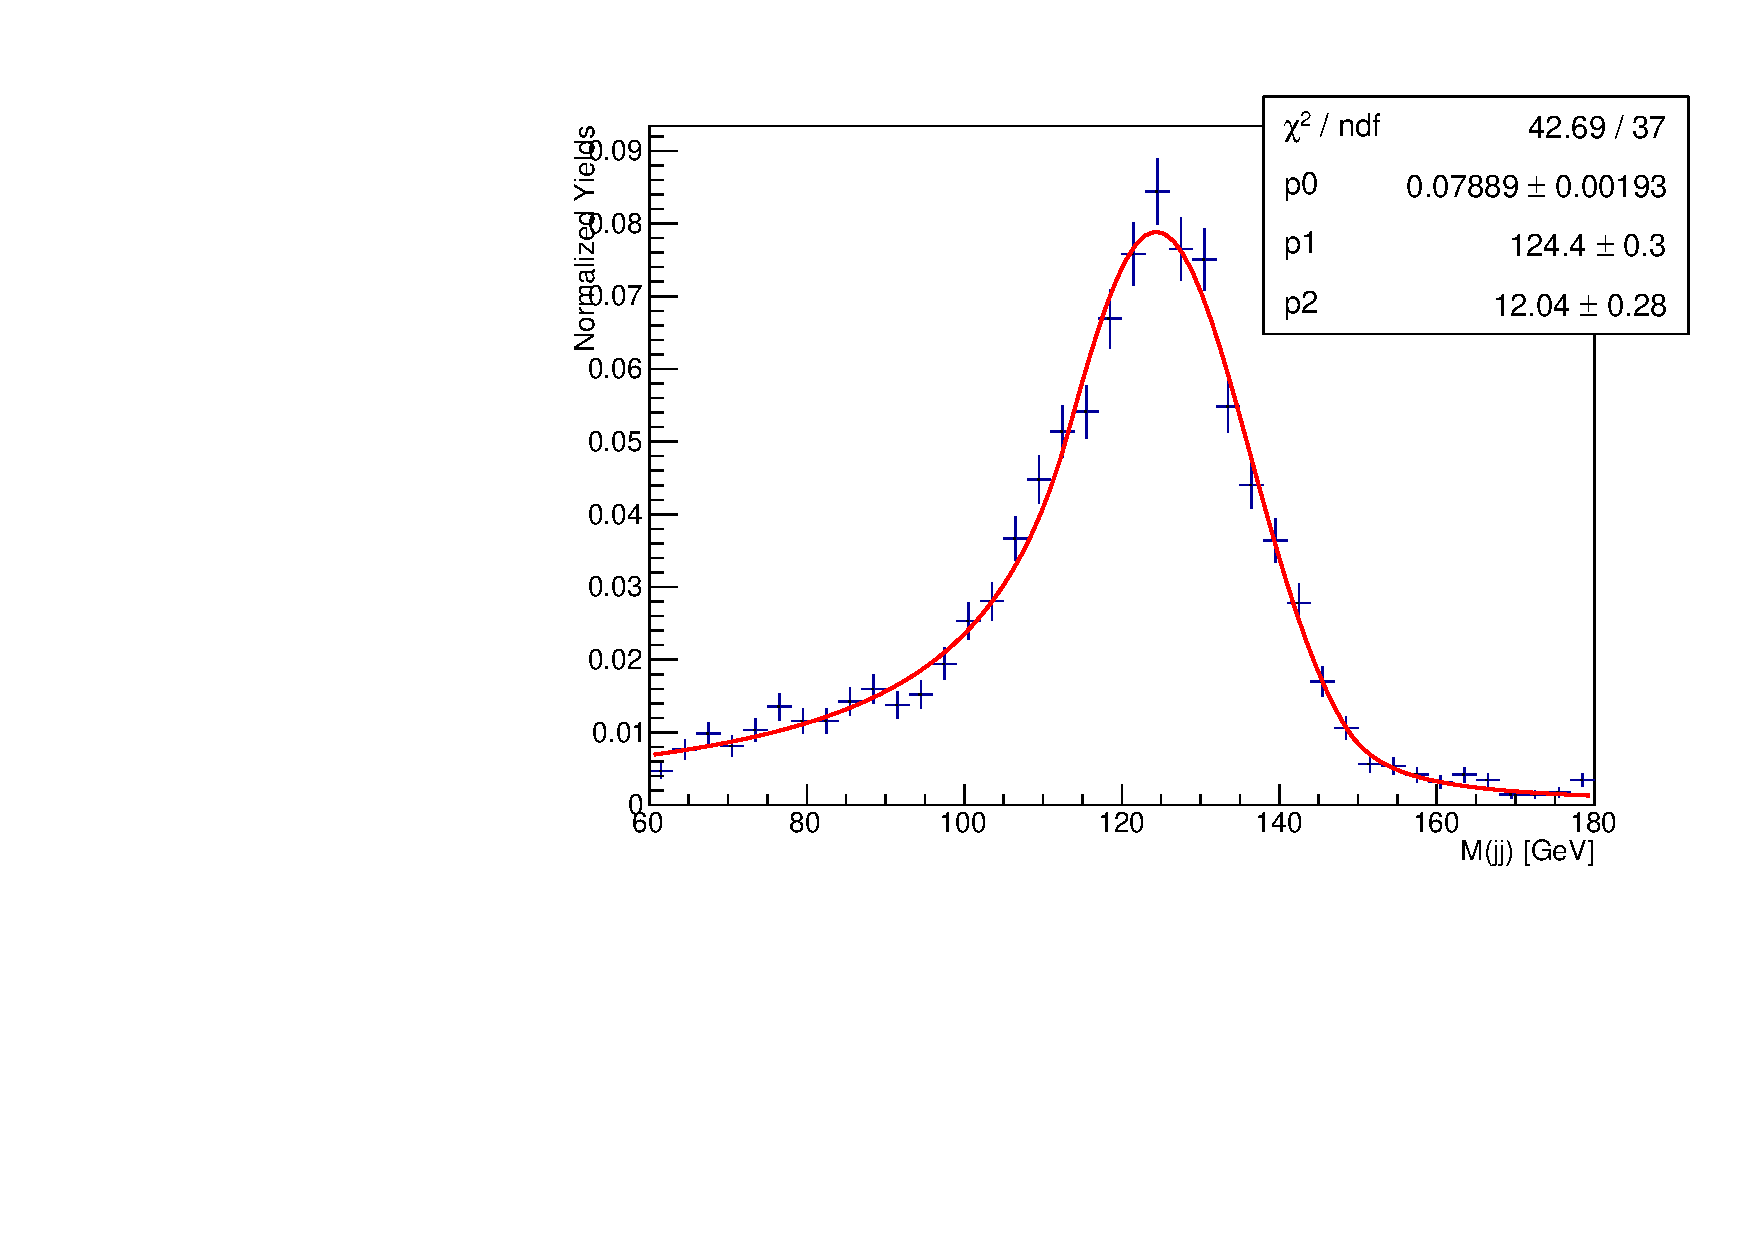
\includegraphics[width=0.45\textwidth]{figures/sec-systematics/mjjHMMPC_fixed_up.pdf}\hfil
  \caption{Signal fits for the High Mass Medium Purity category, in the un-smeared MC with floating tails (left) and on the smeared MC with fixed tails (right). The tail parameters on the right are fixed to their values on the left.}
  \label{fig:mjj_smear}
\end{figure*}

\begin{figure*}[h]
  \centering
  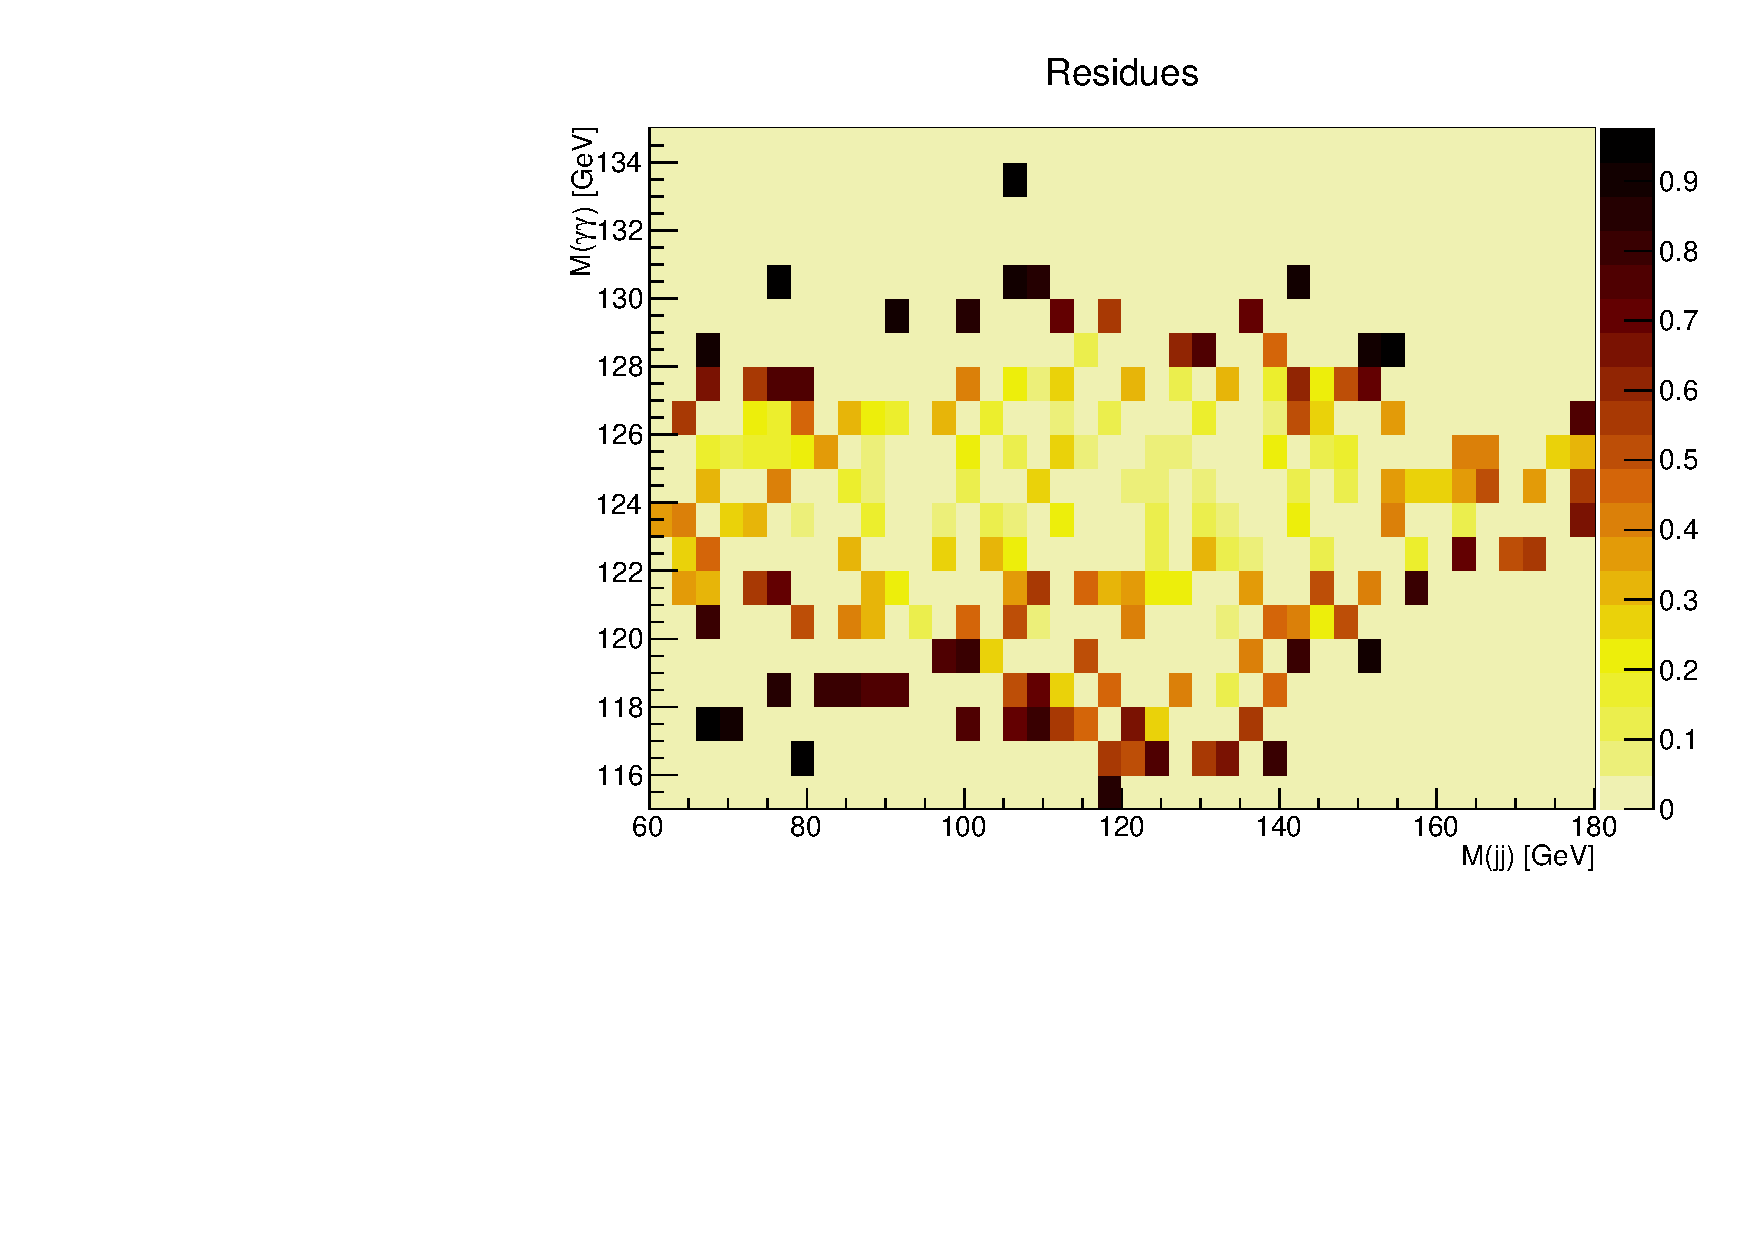
\includegraphics[width=0.45\textwidth]{figures/sec-systematics/HMMPC_up_tails_notfixed_central_res.pdf}\hfil
  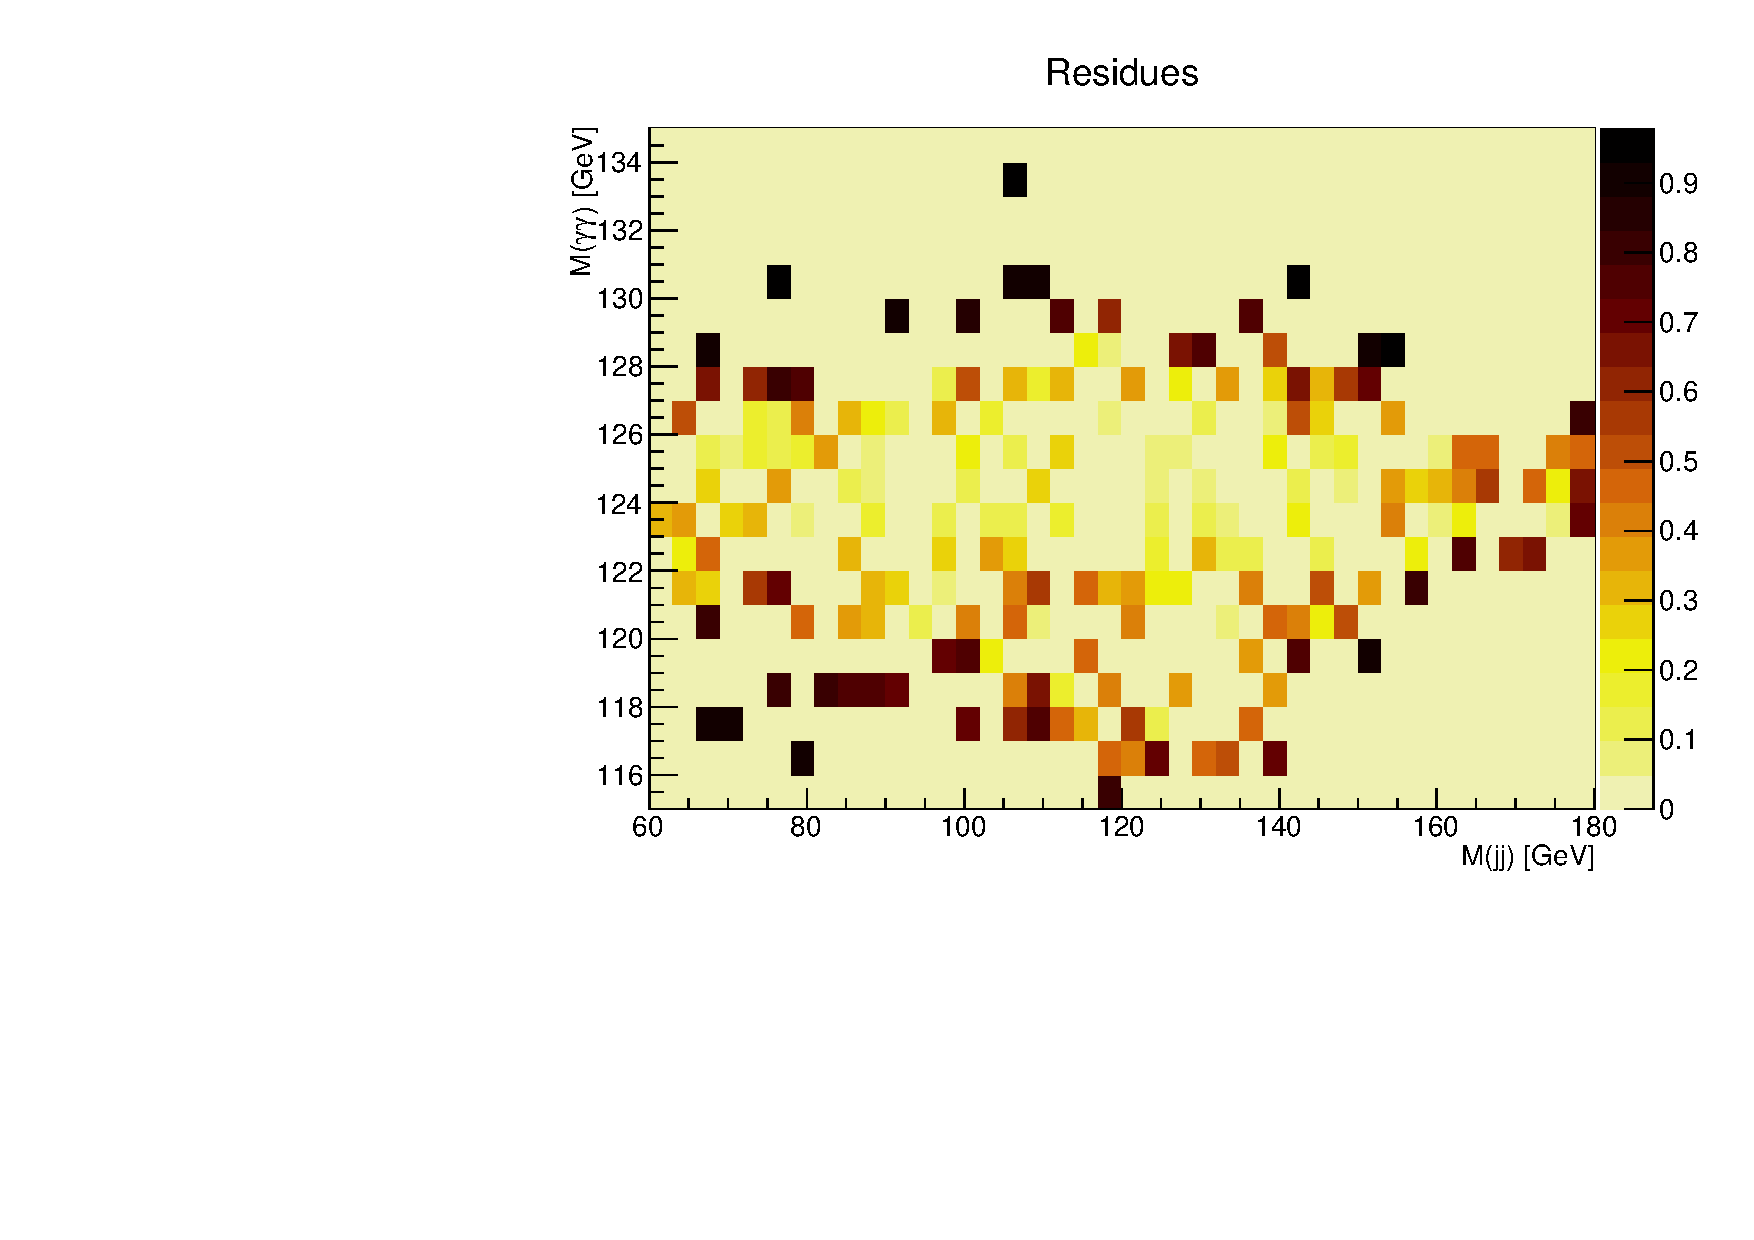
\includegraphics[width=0.45\textwidth]{figures/sec-systematics/HMMPC_up_tails_fixed_central_res.pdf}\hfil
  \caption{Residuais comparing the floating signal PDF fit to the smeared MC (left) and the fixed tails PDF fit to the smeared MC (right) in the High Mass Medium Purity category.}
  \label{fig:res_smear}
\end{figure*}

\begin{figure*}[h]
  \centering
  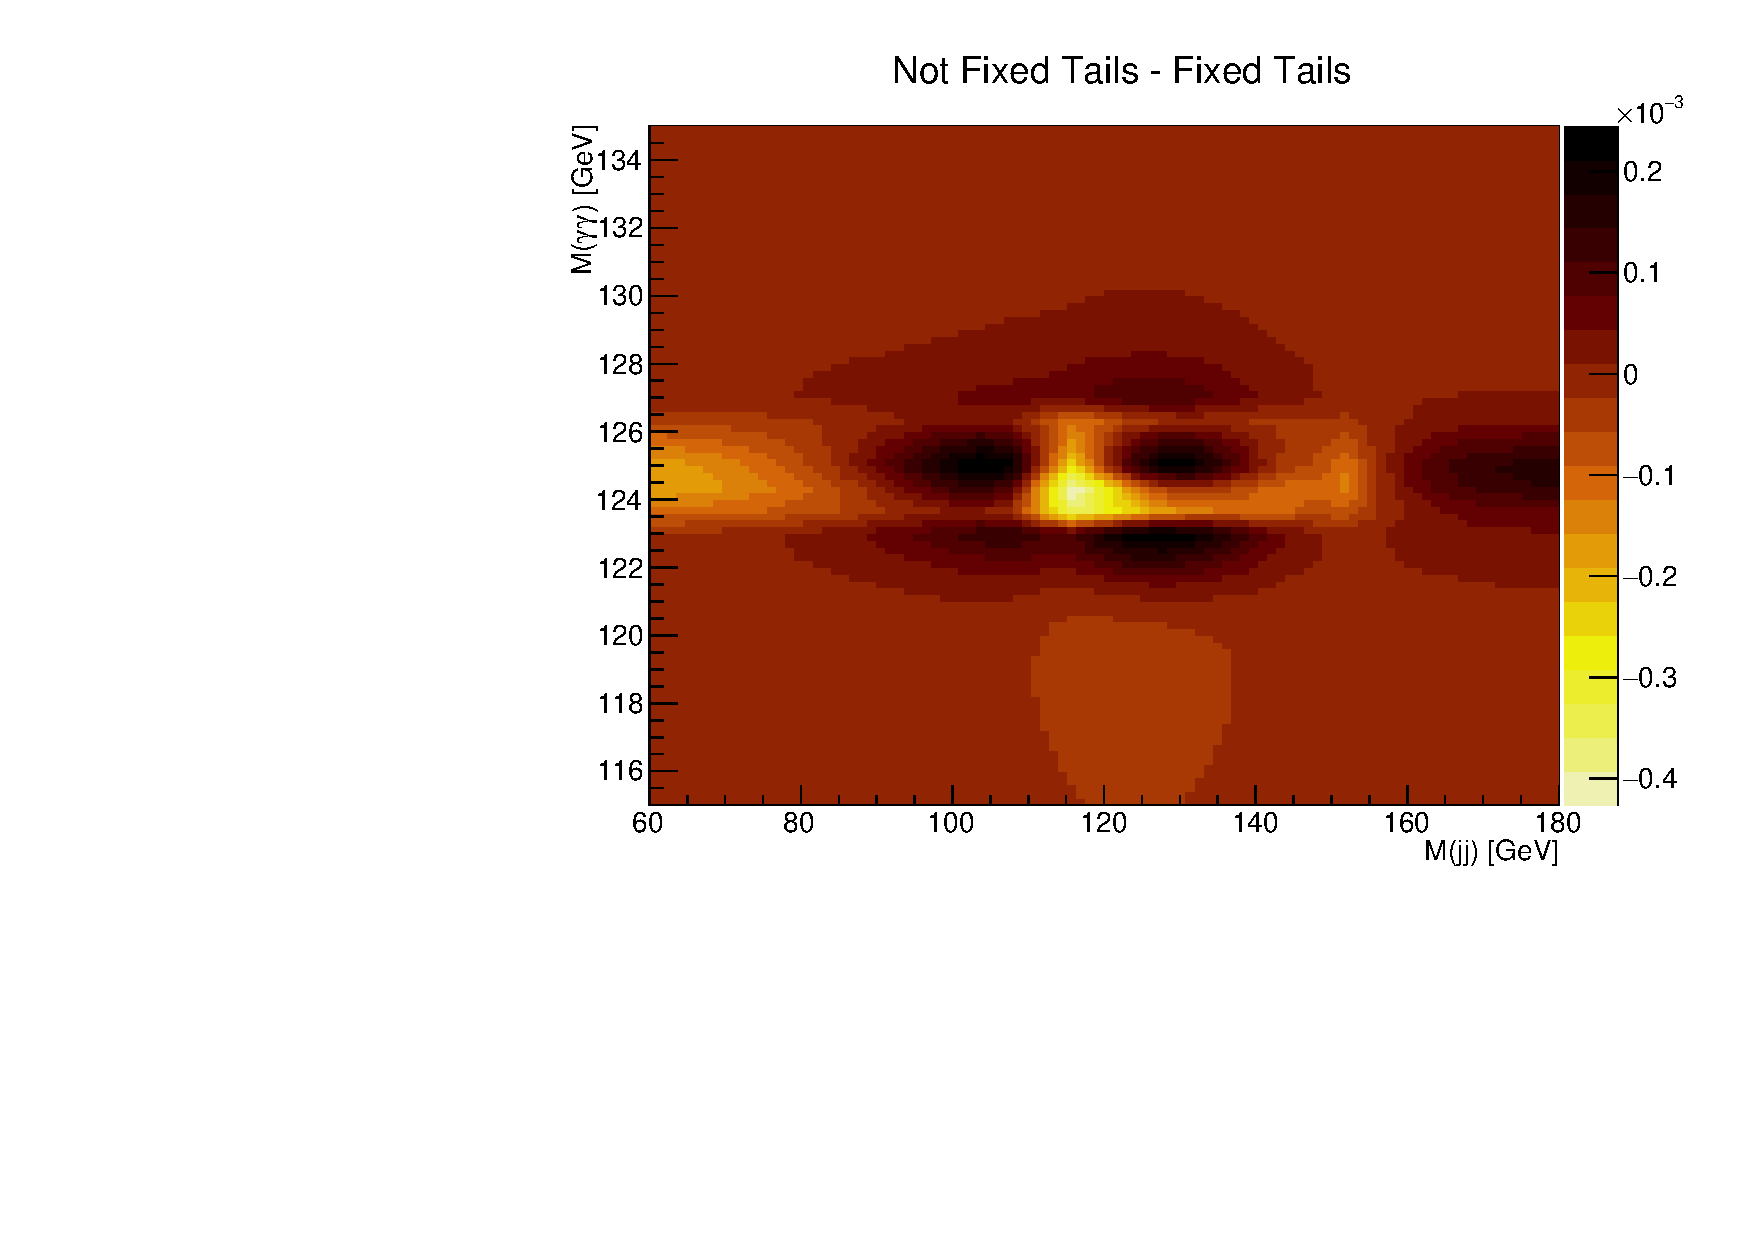
\includegraphics[width=0.45\textwidth]{figures/sec-systematics/fixnfix.pdf}\hfil
  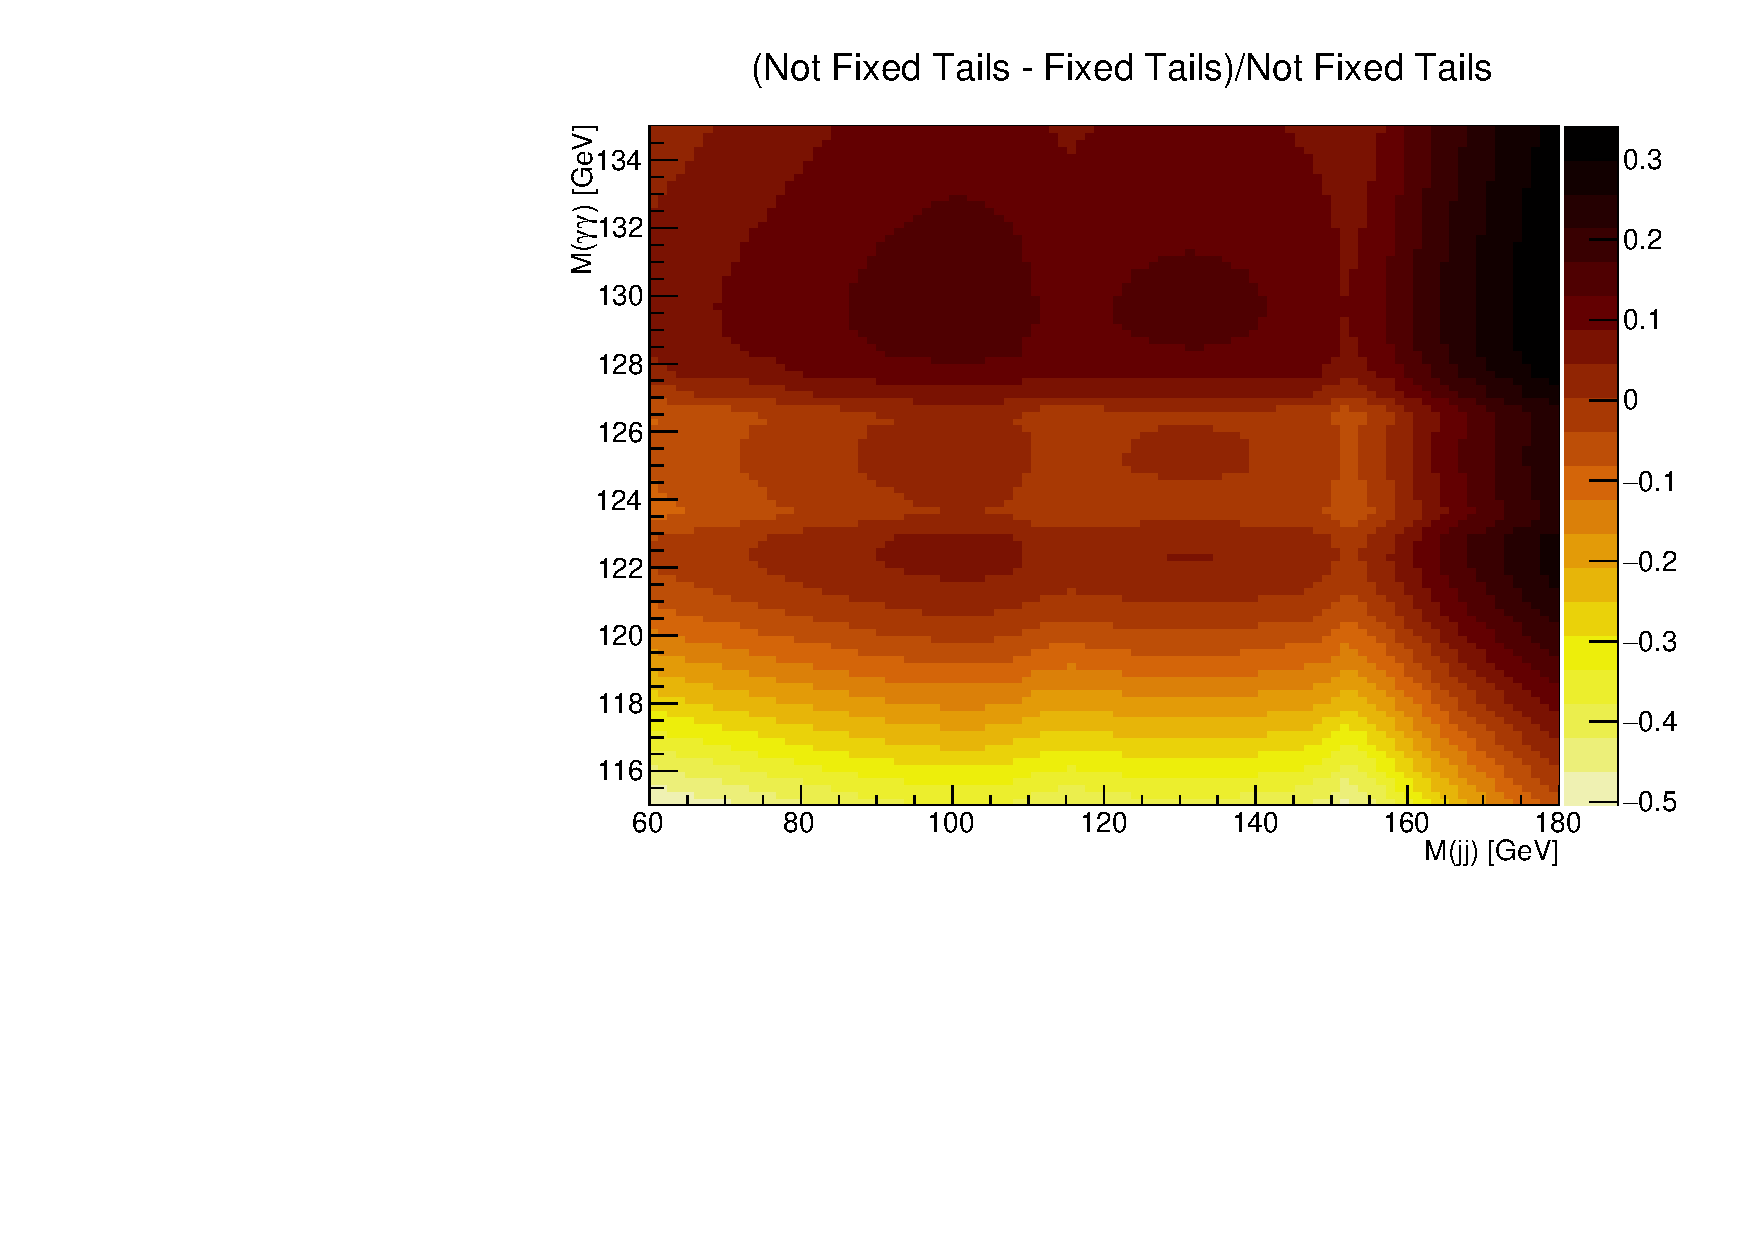
\includegraphics[width=0.45\textwidth]{figures/sec-systematics/fixnfixE.pdf}\hfil
  \caption{Comparison between fixed and floating PDF shapes when fitting the smeared MC.}
  \label{fig:comp_smear}
\end{figure*}

